%! Author = guney
%! Date = 03-Aug-25

% Document
\section{Modeling Methodology}\label{sec:modeling-methodology}
\subsection{Overview}\label{subsec:overview}
    MacroSim bases its discovery process on top of a simple $AR(n)$ process where $n$ defines the number of lags for the target variable.
    The constant $c$ and error term $\epsilon$ are assumed 0 and inclusion of noise and linear offest is offloaded to the discovery engine.
    \\

    To aid discovery, supplementary variables are selected from the feature space through the use of \href{https://en.wikipedia.org/wiki/Granger_causality}{ Granger Causality Tests (GCT)} and \href{https://en.wikipedia.org/wiki/Augmented_Dickey%E2%80%93Fuller_test}{Augmented Dickey–Fuller Tests (ADF)}.
    This creates a set of variables that are either direct lags of the target, or are both stationary and have a Granger causal relationship with the target.
    \\

    A symbolic regressor (SR) is responsible for patching these variables in a meaningful way while fitting the AR weights simultaneously.
    Denoting the target as $y$ and the supplementary features as $X_i$, the ultimate resulting expression follows the form $f(AR_y(n), X_1, \dots, X_i)$.
    This process applied to all variables in the feature space to produce a complete and self-sustaining simulation model.

\subsection{Data Preparation}\label{subsec:data-preparation}
\subsubsection{Collection and Formatting}
    MacroSim requires a dataset of time series with matching dates and frequencies.
    There are methods implemented to get, re-index, impute, and format data directly through methods supplied in the library\footnote[1]{See \autoref{subsec:module-structure}\label{fn1}}.
    The data is expected to be in a \texttt{pandas.DataFrame} with a \texttt{DatetimeIndex} and is expected to be entirely numeric.
    There are no expected encoding specifications for categorical variables, but symbolic regression may yield better results with \href{https://en.wikipedia.org/wiki/One-hot}{One-hot Encoding} due to the possibility of having individual coefficients for each category.

\subsubsection{Splitting}
    The target variable is passed to the \texttt{AutoReg} class as a string.
    The processing steps of splitting the features, and creating train/test splits are handled internally.
    \texttt{AutoReg} contains methods to batch and shuffle the data to prevent overfitting due to ordered data and utilize an ensemble learning technique for further robustness.

\subsubsection{Inter-Process Data Transmission}
    Due to the limitations with the dependencies of \texttt{MacroSim}, creating thread pools with shared memory is not possible.
    To allow true parallelism, \texttt{\_batch\_fit} and \texttt{AutoReg} communicate by stripping the non-serializable portions of the model and its output.
    This effectively destroys all but the fitted equation as a string and some limited metadata.
    The equations are converted to \texttt{sympy.Expr} objects and serialized through \texttt{pickle}.
    Upon loading the equations, the metadata is used to reconstruct the model as a native python callable through \texttt{sympy.lambdify}.
    \\

    \texttt{\_Predictor} and \texttt{\_BatchedPredictor} classes wrap these callables and define the standard methods expected to exist in a fitted model.
    (mainly \texttt{predict} and some scoring functions)

\subsection{Target Lag Selection}\label{subsec:target-lag-selection}
    By default, lags of the target feature are configured to cover a 2-year period of observations.
    (two complete cycles of seasonality in many economic contexts)
    This is adjustable through the \texttt{AutoReg.n\_lags}\footref{fn1} attribute, which will be automatically populated with the default lag count using the formula $n_{lags}=2s$ where $s$ denotes the inferred yearly observation frequency.
    \\

    Importantly, lag generation causes data to be shifted, which results in a loss of the first $n_{lags}$ observations.
    Alongside other processes such as training and testing set generation, this can lead to a sizable decrease in usable observations.

\subsection{Feature Selection}\label{subsec:feature-selection}
\subsubsection{Granger Causality}
    By definition, Granger causality tests the predictive power of a variable's past values on the current value of the target.
    Informally, the test structure can be denoted as follows:
    \begin{gather*}
        H_0: X_{t-i} \cancel{\underset{\text{granger-causes}}{\to}} y\\
        H_1: X_{t-i} \underset{\text{granger-causes}}{\to} y\\
    \end{gather*}

    GCTs can take bivariate and multivariate forms; however, MacroSim strictly uses the bivariate form.
    Multivariate GCTs deem if a pair of variables Granger cause the target, but present no further information on the significance of the individual variables.
    This structure necessitates making assumptions to assess and score each variable.
    \\

    Multiple test statistics can be used to determine the significance of the relationship, such as the F-statistic, Chi-squared statistic, and the likelihood ratio.
    MacroSim adopts the F-statistic and performs local causality tests over slices of the data.
    The slices are sized to cover an 8-year period, and the \texttt{max\_lag} parameter is dynamically set through the formula:
    \begin{equation*}
        max\_lag = \nint*{\frac{N_{obs}}{20\cdot freq}\cdot \ln (N_{obs})}
    \end{equation*}

    This formula provides an almost linear increase in lag size for larger datasets, while smaller datasets receive more conservative lag sizes.

    \begin{figure}[h]
      \centering
      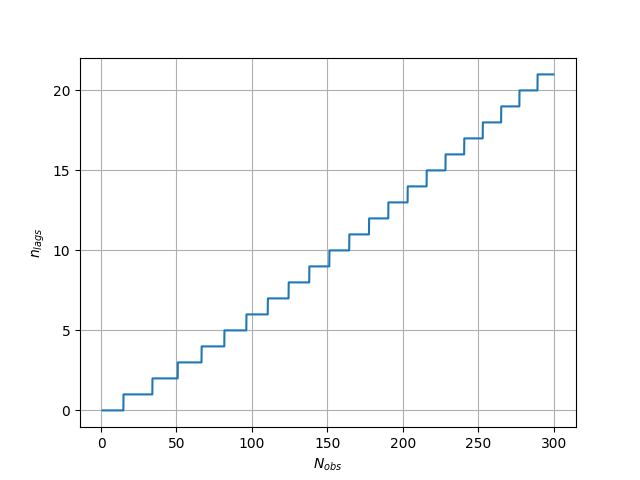
\includegraphics[width=\linewidth]{./assets/Figure_1}
      \caption{Function output for quarterly frequency up to 300 observations.}
      \label{fig:quarterly-output}
    \end{figure}

\subsection{Equation Discovery}\label{subsec:equation-discovery}
    \dots

\subsection{Recursive Simulation}\label{subsec:recursive-simulation}
    \dots



